\chapter{Network Models}\label{chapter:network_models}


In this chapter, we present and formally describe two classes of network models that were developed during this study.
\textbf{Species-collector networks} (SCNs) are built based on associations between collectors and the species they have recorded based on their field activities, whereas \textbf{collector coworking networks} (CWNs) describe direct collaborative associations between collectors when recording specimens in the field.

Although structurally distinct, SCNs and CWNs provide complementary perspectives on the recording behavior of collectors from a given species occurrence dataset. 
From SCNs, we retrieve information on which collectors have recorded which species and, conversely, which species were recorded by which collectors. 
On the other hand, CWNs allow us to investigate which collectors team up with whom during fieldwork, although here species are not represented as entities.
As both network models were elaborated based on a framework for social network analytics, we first review some general concepts from the network science and graph theory domains that are used in this study.

% ======================
% ======================
% Network Science Theory
% ----------------------

\section{Network science: A theoretical background}

Network science refers to a relatively new domain of scientific investigation, which aims at describing emergent properties and patterns from complex systems of interacting entities.
Such relational systems are naturally represented as networks, in which interactions are represented as pairwise connections (\textit{links}) between entities (\textit{nodes}) and assume particular semantics depending on the nature of the modeled phenomenon.
The rise of this field is strongly associated with recent advances of information technology, which provided scientists with novel tools for collecting, storing, and processing data from many knowledge domains in a more efficient way and at larger scales.
Although a variety of networked systems in many disciplines have been studied long before that, technological advances allowed the modeling of real-world systems in much more details, from large volumes data that are often public or easily accessible for the investigators.


In a seminal $1999$ paper that has inspired many researchers to engage into the field of network science, \textit{Albert-László Barabási}, \textit{Hawoong Jeong}, and \textit{Réka Albert} built a model of the World-Wide Web from data collected by a web crawler~\cite{Albert1999}. 
Their model represented the web as a set of interconnected documents, where a connection between document $a$ and document $b$ existed if either $a$ contained hyperlinks pointing to $b$ (outgoing links of $a$) or if $a$ was referred by $b$ through hyperlinks (incoming links of $a$).
By exploring some of the model topological features, they estimated that although the web is composed of a huge number of documents (by that time there were around $8 \times 10^8$ documents online), two randomly chosen documents are, in average, separated by a relatively small number of links (19~in their study). 

Although surprising, this finding was in fact consistent with a generative model proposed by \textit{Watts} and \textit{Strogatz} in $1998$ \cite{Watts1998}.
In that paper, authors argued that real-world networked systems are neither completely randomly nor completely regularly connected, and demonstrated that more realistic topologies could be derived by combining features from both extremes.
Following this approach, they were able to generate network models which became known as the \textbf{small-world networks}, in which nodes are separated from others by very few connections, even for very large systems, while still keeping a relatively high clustering structure.
% \art{Lembre-se que redes small-world combinam simultaneamente a diametro pequeno E clustering alto.}
This kind of networks was named after a phenomenon known as \textit{small-world}, which became popular after the experimental work of \textit{Stanley Milgram} \cite{Milgram1969} that also led to the expression ``six degrees of separation''.
The concept referred to the experimental finding that two arbitrary individuals in a large population are separated by at most 6 connections, following an acquaintances chain~(i.e. a relatively low number of connections compared to the population size).

Besides the small-world network model, other models have been proposed in literature to explain mechanisms by which real world networks grow and acquire topologies with particular properties.
A \textit{preferential attachment mechanism} was proposed by \textit{Barabási} as ruling network growth by preferentially connecting new nodes to those in the network that already have many connections \cite{Barabasi1999a}.
This phenomenon is also referred to as ``the rich gets richer'' effect and allows the appearance of few heavily connected nodes in the network, called \textit{hubs}. 
The majority of nodes in the network are, in contrast, very poorly connected, and thus unlikely to be linked with the new edges.
Large networks with such characteristics are also known as \textbf{scale-free networks}.

Those recently proposed models represent advances if compared with a \textbf{random network model} as the $G(N,p)$ model by \textit{Paul Erdos} and \textit{Alfred Rény}~\cite{erdos1959random}. In the $G(N,p)$ model, 
random networks are generated by creating $N$ distinct nodes and each pair of nodes is connected with a uniform probability $p$, independently of the number of connections a node already has. 
In random networks, topologies in which few hubs coexist with a massive amount of very poorly connected nodes are then extremely unlikely to be observed. 
% \art{Cuidado. Existem redes reais com caracteristicas mais proximas de redes aleatorias.}


Empirical results thus indicate that links are not randomly established in many real-world networks.
Instead, plenty of system-specific mechanisms occurring in smaller scales are thought to be key in the process of link creation.
Network growth is thus not governed by a global mechanisms, but results from the orchestration of many local processes that occur between entities within the system.
We refer to such networks, in which non-trivial topological features emerge from the dynamics of subcomponents, as \textbf{complex networks}.
Uncovering some of such mechanisms and characterizing their effects in network topology compose the core of network science.


%% Examples of networks in biology, computer science...
Network science has been applied to model networked systems in a variety of knowledge domains, including the Internet, movie actors costarring networks, scientific collaboration networks, networks of human sexual contacts, cellular networks, and ecological networks just to cite a few \cite{Albert2002}.
Given their relational structure, network models are formally represented as \textbf{graphs}.

Next we briefly review some fundamental definitions from \textit{graph theory}.
For the purpose of this work, this is not intended to be a thorough review on the subject, but rather a quick overview for not familiarized readers. 
For a slightly more comprehensive introduction we recommend the reader to refer to \textit{Barabási}'s and \textit{Newman}'s books on network science \cite{Barabasibook,Newman2010b}.
In the sequence, we briefly describe the social network analytics framework and, 
finally, we give some examples of applications of network thinking in the biodiversity literature.


% ============
% Graph Theory
% ------------
\subsection{Some concepts from graph theory}
\label{section:graphtheory}

Intuitively, \textbf{graphs} are mathematical structures composed of discrete objects holding pairwise connections to each other. 
In graph theory terminology, objects are referred to as \textit{vertices} and the connections between them as \textit{edges}.
Graph structure provides a natural representation for networked systems for a couple of reasons.
First, they allow representing entities and their interactions in a structured way, as a ``map of connections'' through which information flows.
Second, graph theory provides a bunch of well established data structures, metrics, and algorithms for systematically representing, characterizing, and exploring the topologies of complex networks.
Finally, the availability of a considerable amount of graph visualization tools and techniques helps analysts to obtain insights from network structures by allowing them to focus on different aspects of the networked complex system depending on their own interests.


% Graph formal definition, undirected/weighted graphs
A graph is formally defined as a pair $G=(V,E)$, where $V$ is the set of vertices and $E$ is the set of edges that compose the graph~(Figure~\ref{fig:graphs}). 
%
Edges typically involve pairs of vertices and are thus represented as $(u,v)$, for $u,v \in V$.
Pairs of vertices that are directly connected by an edge are said to be \textit{adjacent}, and the set of all vertices that are adjacent to a given vertex composes its \textit{neighborhood}.
%
Depending on the nature of the modeled connections, edges can be either classified as \textit{undirected} or \textit{directed}.
Undirected edges model symmetric connections, in which case information is allowed to flow equally in both directions.
There are situations, however, in which information necessarily flows from a source to a target vertex, thus making connections asymmetric.
Those are represented in the graph as directed edges.
Graphs strictly composed of directed edges are known as \textit{digraphs} (or \textit{directed graphs}), whilst \textit{undirected graphs} only have undirected edges.
In undirected graphs, we should note that edges $(u,v)$ and $(v,u)$ are equivalent.
%
Additionally, connections in a networked system can be modeled as either being all identical or distinct in terms of their strength or relevance, which is incorporated in the graph as \textit{weight} in the edges.
Graphs are also classified regarding the nature of their edges.
A graph in which all edges are weighted is known as a \textit{weighted graph}, whilst a \textit{unweighted graph} is exclusively composed of unweighted edges.
%
Given the nature of the networks modeled in the context of this project, we specifically focus on properties of \textbf{undirected weighted graphs} for the rest of this section.


\textit{Attributes} allow representing non-topological features that are relevant in the context of the modeled networked system, and can be optionally assigned to both edges and vertices in a graph.
For example, we might want to model a social network in which age and gender information about individuals are relevant for the intended analyses.
Such features, which assume distinct values for each individual in the network, are typically stored as attributes of the vertices.
Similarly, edge attributes store particularities regarding each individual connection between a pair of vertices.
In principle, any numerical edge attribute could be used for weighting edges.

% Graph representations
Graphs can be computationally represented using a variety of data structures, the most appropriate one heavily depending on the set of algorithms one expects to run using the graph.
Figure \ref{fig:graphs} shows an illustrative undirected weighted graph and three of its possible representations: an edge list, an adjacency matrix, and an adjacency list, which are explained next.

\begin{figure}[h!]
  	\centering
    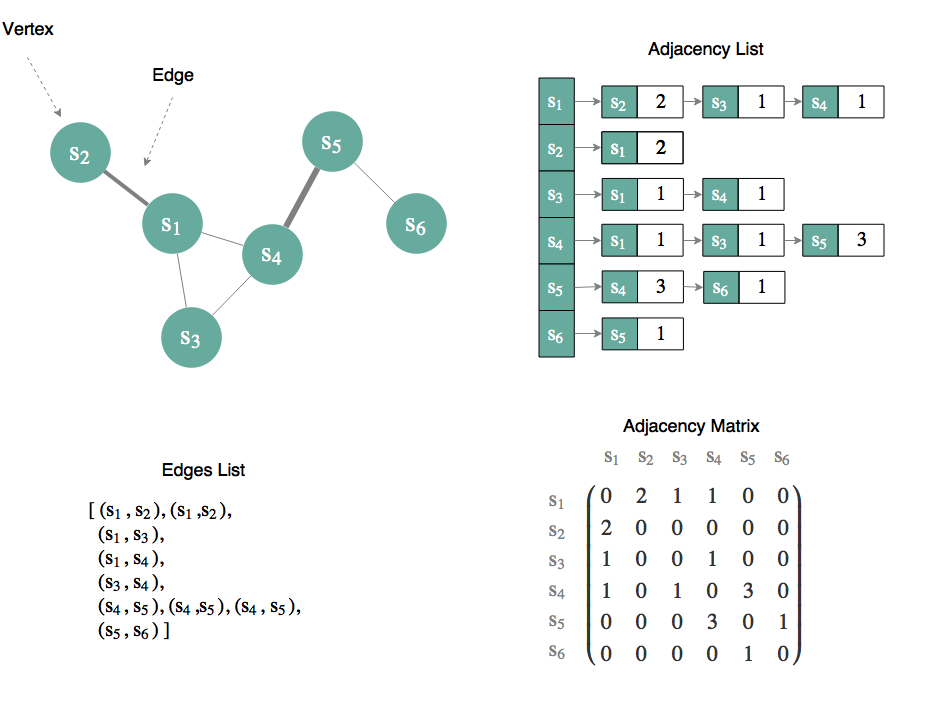
\includegraphics[width=0.9\linewidth]{figures/network_models/graphs.png}
    \caption{Undirected weighted graph with six vertices and six edges (the thickness of an edge represents its weight); and three of its possible representations.}
    \label{fig:graphs}
  \end{figure}
  

\textit{Edge lists} are possibly the simplest and most intuitive graph representation, consisting of a list storing all edges as ordered pairs $(u,v)$, for $u,v \in V$.
Given its simplicity, this representation is more appropriate for situations in which the user directly interacts with the data, such as when manually creating or editing graphs without the aid of specialized software. 
This representation is also compact enough to be adopted for graph storage and data exchange in some situations.
%
Most algorithms, however, perform better by using alternative representations, such as \textit{adjacency lists} or \textit{adjacency matrices}. 

\textit{Adjacency matrices} are a way of representing graphs in matrix form, in which elements store adjacencies between pairs of vertices.
An adjacency matrix $A$ is defined as having non-zero entries $a_{i j}$\textit{ if, and only if } $(i,j)\in E$ which, in weighted graphs, correspond to the weight assigned to edge $(i,j)$.
Given the equivalence between edges $(i,j)$ and $(j,i)$ in undirected graphs, adjacency matrices in this case are always symmetric, meaning information is stored redundantly in its structure.
%
Besides, the size of an adjacency matrix grows quadratically with the number of vertices in the graph, which would make loading and processing large graphs in computer memory problematic.
However, real-world networks have been observed to be naturally sparse, meaning that only a very small percentage of all possible edges do in fact exist.
Adjacency matrices can thus be optimized for storage and performance by adopting standard sparse matrix representations, such as compressed row storage~(CRS)~\cite{Saad2003}.
An alternative way to represent sparse networks is to use the \textit{adjacency list} representation, which in short consists of storing a list of neighbors for every single vertex in the network. 
The adjacency list illustrated in Figure~\ref{fig:graphs} is structured as an array for which each entry represents a vertex.
Moreover, each entry holds a reference for a linked list, containing all neighbors of the vertex. Each element in the list keeps a reference to the next element and stores the weight of the edge connecting it to the vertex in the array.

\luiz{Parei minha revisão aqui}

% Definitions and metrics
As previously mentioned, one of the main benefits of adopting graphs for representing networks is the availability of a whole set of well-established metrics and definitions that allow analysts to explore and characterize the topologies of their networked systems.
We next review some of the main concepts for network analysis that are useful in this dissertation.

\paragraph*{Path.}
A path can be thought of as a chain of adjacent vertices composing a route through which information may flow in a graph.
For undirected graphs, there exists a \textit{path} of length $n$ between a given pair of vertices if they are mutually reachable by following a sequence of $n$ edges.
A pair of vertices is said to be \textit{connected} if at least one path exists between these vertices. The shortest path between a pair of vertices is defined as the \textit{distance} between these vertices.
%A graph can be described in terms of its \textit{average path length}, which is computed by averaging the path lengths between all pairs of connected vertices.
Finally, the \textit{diameter} of a graph is given by the largest distance between any pair of vertices composing it, although some authors alternatively define \textit{diameter} of a graph as the average length of all the shortest paths between the pairs of vertices.

\paragraph*{Connected component.}
A connected component is a subset of vertices in the graph in which all included vertices are \textit{connected} to every other one by at least one path.
Moreover, this subset is required to be maximal, meaning that all vertices in the network for which the inclusion property holds should also be included in the component. 
A graph can be composed of many distinct connected components completely disconnected from each other. In the case of a graph with more than one distinct connected component, if one of this components comprises the majority of the graph nodes, then this component is called the \textbf{giant component}.

\paragraph*{Clique.}
A clique is a structure composed of a subset of vertices in which all included vertices are \textit{adjacent} to each other.
The set of edges that composes a clique is obtained by computing the pairwise combination of all its $n$ vertices, being the total number of edges in the clique given by the binomial coefficient $\binom{n}{2}$.

\paragraph*{Density.}
Density is one of the simplest metrics for assessing graph connectivity and indicates the proportion of pairs of vertices that are connected by edges.
For a graph with $n$ vertices, density is given by $\frac{2E}{n(n-1)}$, where $E$ is the number of edges in the graph.
Possible values for density are thus limited from $0$ to $1$, where $1$ is obtained for a \textit{complete graph} (or a \textit{clique}) and $0$ would be obtained for a graph with no edges.
This concept is the inverse of graph \textit{sparsity}. 


\paragraph*{Clustering.}
Density alone is seldom a sufficient metric for investigating relevant patterns of connectivity in real-world networks, as their topologies usually display \textit{clustering patterns}.
\textit{Clusters} are regions in the graph in which vertices are significantly more densely connected than average and more loosely connected with other vertices from the reminder of the graph. 
Clustering analysis is particularly useful in the context of social network analysis for identifying communities.
%
\textit{Clustering coefficients} are used to characterize the how clustered vertices are in a graph, and can be defined as either local or global metrics.
The local clustering metric $c_i$ for a given vertex $i$ is calculated by evaluating how close to a clique is a subgraph composed of the vertex $i$ itself and all its $k$ neighbors~(which is known as the \textit{ego network} of vertex $i$). Thus, $c_i = \frac{2L_i}{k_i(k_i - 1)}$, where $L_i$ is the number of edges connected to $i$ and $k_i$ is the degree of $i$.
To illustrate with an intuitive example within the context of social networks, a local clustering coefficient is an answer to the question ``To what extend pairs of my friends are also friends themselves?''.
%
The global clustering metric $c_{\Delta}$, on the other hand, computes the fraction of triplets in the graph that composes cliques of three nodes~(i.e., triangles). A triplet is three nodes that are connected by either two (open triplet) or three (closed triplet) undirected ties. A triangle therefore includes three closed triplets, one centered on each of the nodes. In short, \begin{equation}\label{eq:globalclustering}
c_{\Delta} = \frac{3 \times numOfTriangles}{numOfTriples}.
\end{equation}

\art{Parei minha revisao aqui}


%% Transitivity
\paragraph*{Transitivity.}
The transitivity relation for a triple of nodes $\{a,b,c\}$ is observed if the fact that node $a$ is connected to $b$ and $b$ to $c$ implies that $a$ is connected to $c$.
In social networks terms, this relation represents the phenomenon that ``a friend of my friend is also my friend''.
Network transitivity is often used as a synonym for \textit{clustering}, and thus the overall transitivity of a network can be quantified through the global clustering coefficient from equation \ref{eq:globalclustering}.



\paragraph*{Degree.}
The degree (denoted $k$) of a vertex in a undirected graph is given by the total number of vertices that are adjacent to it or, in other words, the length of its neighborhood.
We compute the degree of a particular vertex $i$ from the graph's adjacency matrix $A$ as 
$
k_i = \sum_j bool(a_{i j})
$,
where $a_{i j}$ are elements containing the weights of each edge $(i,j)$; and the function $bool$ evaluates to $1$ if the element is greater than zero and $0$ otherwise.
We can similarly compute the \textit{weighted degree} for vertex $i$ as $ k_w^{(i)} = \sum_j a_{i j} $.
The \textit{average degree} 
$\langle k \rangle$ 
is a global property of the network, computed by averaging the degree values for each individual vertex $i$:
$\langle k \rangle = \frac{1}{N} \sum_{i=1}^N k_i$.

\paragraph*{Degree distribution.}
The probability distribution of vertices degrees over a graph is known as its \textit{degree distribution}.
From degree distribution we retrieve the probability $p_k$ that a randomly selected vertex from the graph has degree equal to $k$.
In random graphs degree distribution is typically well approximated by a poisson model, which peaks at $\langle k \rangle$.
Thus vertices with degree equal $\langle k \rangle$ are most likely to occur, whereas those with very high and very low degrees are very unlikely. 
As mentioned in the previous section, however, most real-world networks are majoritarily composed by low-degree nodes, coexisting with few hubs.
Such a scenario is better described by a \textit{power law}, such that $p(k) \sim k^{-\alpha}$.

\paragraph*{Degree correlation.}
A graph shows degree correlation if vertices degree determines the degrees of its neighbors with a certain magnitude.
A positive correlation indicates that edges are more likely to connect pairs of either high-degree or low-degree vertices.
On the other hand, a negative correlation indicates that connections are more likely to exist between high-degree and low-degree vertices.
A variety of metrics have been proposed in literature for assessing degree correlation in a graph \cite{Newman2003b}, being the \textit{Pearson correlation coefficient} one of the most widely used.
Generally, correlation values range from $-1$ for maximal negative correlation; to $1$ for maximal positive correlation. 

\paragraph*{Mixing patterns.}
Mixing patterns describe the effects of nodes characteristics on influencing links formation in networks.
In case associations are more likely to establish between nodes which are similar on some characteristic, the pattern is known as \textit{assortative mixing} or, in social sciences, \textit{homophyly}.
In contrast, \textit{dissortative mixing} is observed when nodes preferentially connect to others with opposite characteristics. 
If nodes characteristics show no signifficant influence on links formation, we say the network is \textit{neutral}.
Degree correlation can be understood as a specific type of mixing pattern, evaluated on vertices degrees.

\paragraph*{Centrality.}
Centrality analysis concerns the identification of influential entities in the network, who might assume important roles in the system under different perspectives.
\textit{Degree centrality} is perhaps the simplest centrality measure, and assumes that the relevance of a node only depends on its own degree. Nodes with many connections are thus more influential than those with fewer connections.
If we consider, however, that the relevance of a node also depends on the relative importances of their neighbors (and that some neighbors are more influential than others), the \textit{eigenvector centrality} becomes a more realistic metric \cite{Bonacich1987}.
In this case nodes holding fewer links to more influential ones might turn out to be more influential than those holding more links to less influential nodes.
Other centrality metrics emphasize the importance of other topological aspects instead of node degree.
\textit{Closeness centrality} measures the importance of a node by computing its mean distance to all other nodes in the network, and thus nodes are more influential if they can reach their peers more efficiently by taking shorter paths.
\textit{Betweeness centrality} identifies nodes which are important strategical intermediators, if they are included in the path between many pairs of nodes in the network.  

\paragraph*{Bipartite graphs.}
Bipartite graphs, also known as bigraphs or two-mode graphs, are a special class of graphs composed by two distinct sets of vertices $U$ and $V$, with the constraint that no vertices within the same set are allowed to be adjacent to each other. 
We define bipartite graphs as triples 
$
B = (U, V, E) \mbox{, }
$
where $E$ is the set of edges between vertices from $U$ and $V$.
Using sets theory terms, $U$ and $V$ are both \textit{disjoint} and \textit{independent} sets.
This means vertices must be assigned to exactly one vertices set and, moreover, all edges in $E$ necessarily connect vertices from opposite sets. 
Such features make bipartite graphs particularly useful for representing interactions that only make sense to exist between entities of different classes. 

  \begin{figure}[h!]
  	\centering
    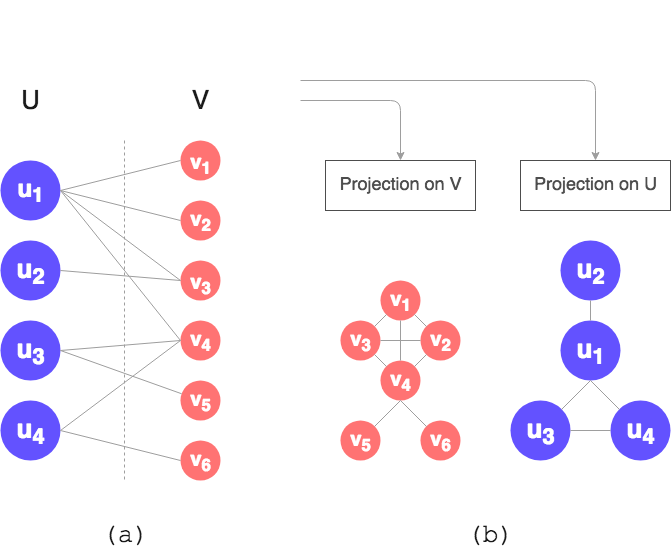
\includegraphics[width=0.5\linewidth]{figures/bipartite_general.png}
    \caption{General aspect of a bipartite graph (a). All vertices in the graph belong to exactly one of $U$ and $V$ vertices sets. In addition edges are only established between vertices from distinct sets. (b) Bipartite projections. Projections onto each node set are constructed by linking together vertices that are at a length-2 distance in the bipartite graph, while omitting vertices from the opposite set.}
    \label{fig:bipartite_general}
  \end{figure}

%% Biadjacency matrix
The \textit{biadjacency matrix} (or \textit{incidence matrix}) is the matrix representation of a bipartite graph, being equivalent to adjacency matrices defined for one-mode graphs (those composed by a unique vertices set). 
Differently from one-mode graphs for which the adjacency matrix is necessarily square, biadjacency matrices are usually rectangular, unless both vertices sets have the same size.

%% Bipartite projection
As most algorithms and metrics in literature are primarily designed for one-mode graphs, it is often convenient to summarize a bipartite graph by directly linking vertices that belong to the same set based on indirect associations they might have. 
This operation, in which vertices from one set get directly linked if they are intermediated by at least one vertex from the opposite set, is called a \textit{bipartite projection} (Figure \ref{fig:bipartite_general}b).
Projections thus compress a bipartite graph into a one-mode graph by only representing vertices from the projected set, while those from the opposite set are omitted.
Therefore, bipartite projections into each vertices set provide complementary perspectives on the relationships modeled.
%




% ===============
% Social Networks
% ---------------
% Mark Granovetter paper (1973)
%% Which types of analyses are most common in social networks?

\subsection{The Social Network Analytics framework}
In the context of this work we refer to the \textit{social networks analytics framework} as a set of concepts, methods and algorithms which can be directly applied or slightly adapted for modeling and analyzing social networks in diverse and independent contexts and knowledge domains.
%
In our definition, we refer to \textit{social networks} as systems in which entities (mostly people) interact with each other through some type of \textit{social tie}.

As social networks are themselves a particular class of networks, most of the theoretical foundation used to study them is directly inherited from network science.
%
Social networks, however, display two important particularities if compared to other types of networked systems \cite{Newman2003d}.
First, entities tend to organize themselves in groups within social systems, such that those who are members of the same group tend to interact more intensely with themselves than with non-members.
This contributes to the formation of communitites structures, making social networks \textit{highly clustered}.
Second, as entities belonging to larger groups tend to interact with many peers --- and, conversely, entities belonging to smaller groups tend to interact with fewer peers ---, social networks tend to be assortatively mixed, in contrast with non-social networks which are typically disassortative.  

%Properties 
A variety of social network models within many distinct areas have been proposed in literature.
Most authors have primarily focused on obtaining domain-specific insights from statistical and topological properties of network models such as \textit{degree distribution}, \textit{degree correlation}, \textit{mixing patterns}, \textit{nodes centrality} and \textit{clustering} \cite{Newman2003b}.
Next we describe some of them for giving the reader a more solid intuition on how they're structured before we introduce our own models.


% Affiliation networks
\textbf{Affiliation networks} are a particular type of social networks in which individuals are associated to events, groups or institutions (we'll refer to all those as organizations) by being members or participating in them \cite{Borgatti2015}. 
%
Such networks are considered relevant in the context of social networks analytics due to the fact that individuals belonging to the same groups or attending the same events are more likely to become acquainted and develop social ties than those who are not affiliated to common organizations.
%
The most conservative way to structure affiliation networks, so that we keep the complete information on who have affiliated to which organizations, is achieved by representing both individuals and organizations as distinct types of entities in a bipartite model.
 
A classic example of affiliation networks is the movie actors network, introduced as an empirical example in \textit{Watts} and \textit{Strogratz}'s work \cite{Watts1998} while describing the small-world property in real-world networks.
This network was built from the Internet Movie Database (IMDB \footnote{\url{http://www.imdb.com/}}), by linking actors to movies they have starred in.
Actors and movies are thus modeled as distinct entities in the network, such that an actor gets connected to all movies he/she has participated in, whilst a movie gets connected to all actors who have composed its cast.  
From complementary perspectives, one could distinguish for instance movies that are most similar in terms of their cast composition and, on the other hand, actors that are most related by having starred in the same sets of movies.
%
Similarly, \textit{Davis}, \textit{Garder} and \textit{Gardner} have studied women social circles from data on their attendance to public social events, and related how their attendance behavior could be influenced by their own social casts \cite{Davis1941a}. 

Another well-known application of affiliation networks are scientific papers authorship networks, in which authors get connected to papers they've authored.
In this case, however, the focus has been mostly on deriving co-authorship relationships between paper authors, and in many cases the individual papers which originated the co-authorships are not very relevant \cite{Newman2004, Borrett2014}.
A simplified one-mode network, in which only authors are represented as nodes and get directly linked by co-authorship relations, can be derived from the bipartite model by computing its projection onto the authors nodes set.
In the resulting network, authors who have collaborated at least once in paper production get directly connected.
Networks where edges assume this semantic are also known as \textbf{collaboration networks} (or, alternatively, \textit{coworking networks}) \cite{Ramasco2004}.
They can either be directly constructed from data or be obtained by projecting affiliation networks.

Apart from affiliation networks, the bipartite structure is also suitable for modeling other types of social networks.
One of those, which we here refer to as \textbf{interest networks}, model relations of interest from entities towards objects.
Besides their structural similarity to affiliation networks, relationships modeled in interest networks are conceptually distinct from the former, as the fact of two individuals sharing interests does not necessarily provide them differentiated opportunities for developing social ties.
Instead, interest networks tie together individuals with objects they're interested in, independently of the social groups or communities they are members of. 
Thus, instead of social communites, interest networks are more appropriate for revealing {\textit{communities of interests}.
%
Interest networks have been used for instance to characterize collective music listening habitats among users of media streaming platforms \cite{Lambiotte2005}.
From a network of listeners interests towards music groups, \textit{Lambiotte} found evidence that the traditional music genres classification by the music industry is not the best way to categorize listeners in terms of their listening behaviors.



% ========================
% Networks in Biodiversity
% ------------------------
\subsection{Networks in Biodiversity}
Network modeling has been widely adopted in the context of biodiversity research, especially for investigating ecological and evolutionary aspects of ecosystems and natural communities. 
Efforts towards this goal have led to the creation of the field of \textit{network ecology}, which has undergone a noticeable growth over the last few years \cite{Borrett2014}.
% Interaction networks
Network ecology has traditionally focused on describing general aspects of the entangled networks by which organisms interact.
As ecological interactions are regarded as key processes modeling ecosystems functioning and structure, unraveling their architecture and dynamics is essential for understanding a variety of ecosystem features, such as stability and energy flow.
%
Interaction networks can be broadly classified as \textit{food webs}, \textit{host-parasitoid webs} or \textit{mutualistic webs} \cite{Ings2009}, being food webs the first ones described in literature, since two classical papers by \textit{Lindeman} and \textit{Odum} \cite{lindeman1942trophic, odum1956primary}. 
%

%Animal movements
Besides ecological interactions, network thinking has also been applied for modeling other aspects of natural systems.
Patterns of animal movement can be investigated in a structured way, for instance, by means of \textit{movement networks} \cite{Jacoby2016a}.
These networks represent geographical space as a set of discrete and interconnected locations, forming a mesh of possible routes through which animals (or groups of animals) transitate. 
Links between each pair of locations are weighted according to their geographical connectivity.
Animal movement is thus regarded as dynamic processes composed by sequences of discrete movement steps running through the network structure.
As the spatial feature is key in this type of network, they are also referred to as \textit{spatial networks} \cite{Bascompte2007}.
%

%%% Co-occurrence networks 
Others have applied network science to investigate biogeographical patterns, such as species co-occurrence. 
So called \textit{co-occurrence networks} model species associations in terms of their geographical distributions, such that species which are often observed occurring together in the same set of localities are considered to be strongly associated.
Similarly to other networked systems, co-occurrence networks are composed by a majority of the species holding co-occurrence links to very few others, whilst only few species are connected to many others \cite{Araujo2011a}.
Co-occurrence network analysis has been used for many applications, including for selecting subsets of species to be used as surrogates for the characterization of biological communities \cite{Tulloch2016};
for assessing the resilience of biotic communities towards climate change \cite{Araujo2011a};
and for identifying modularity (clusters of overlapping species ranges) in biological communities from animal-location bipartite networks \cite{Thebault2013}.
%%% Challenge: Reliable data is hard to be obtained


% Social Networks and Biodiversity
The social network analytics framework has also been applied in some biodiversity studies, though in most cases for modeling animal social behavior \cite{faust2011animal}.
An alternative perspective is to look at communities of biodiversity data producers and consumers, in order to better understand the myriad of contexts in which data is collected, shared and used.
%
Mapping data flow within the community of biodiversity informatics initiatives, for instance, could help prioritizing and improving the coordination of collaborative actions, leading to more effective biodiversity data-based policies \cite{Bingham2017}.
%
Also, important scientific communities and gaps could be identified and characterized by exploring collaborative paper authoring networks and scientific topics networks \cite{Borrett2014}. 
%
Another interesting example of a collaboration network in biodiversity is given in \textit{Groom`s} work, where a correspondence network of $19th$-$20th$ century botanists was structured from digitized data from the British Herbaria \cite{Groom2014}.
Botanists composing this network corresponded to each other by exchanging specimens, a practice that has led to the formation of exchange clubs.
Many aspects regarding the particular ways botanists used to work as well as the roles they assumed could be investigated with the aid of exchange networks 

% TODO Is this the best way to place this paragraph?
Finally, a better understanding of the factors and processes influencing the composition of species occurrence datasets would be invaluable for improving data usability, especially for species distribution modeling \cite{Daru2017}.
As biological collections are typically composed by an ensemble of opportunistic species occurrence records, each of which having been gathered in a particular context by a different collectors team, their datasets do not necessarily reflect the biological diversity from the area within which the collections are physically located.
Rather, they best reflect the interests of their most relevant collectors, those who have contributed to the collection to greater extents. 
%
In our work we understand the assemblage of a species occurrence dataset as a social process, resulting from a multitude of complex interactions between individual collectors, each of them having particular preferences towards recording taxonomic groups and collaborating with other collectors.
The network models we propose in the following section help characterizing collectors in terms of their interests and recording behavior, as a proxy for a better understanding on the assemblage of biological collections.
  




% ===========================
% ===========================
% Species-collectors Networks
% ---------------------------

\section{Species-collectors Networks}

In this section we introduce species-collector networks (SCNs), which provide the structure for modeling associations between collectors and species they record. 
We first give an overview on the semantics of the modeled relationships and provide a formal definition of SCNs using graph theory, and then we describe how such networks can be built from species occurrence datasets.
Finally, we define attributes and operations for SCNs that facilitate obtaining domain-specific insights from network structure.

\subsection{General Description}
%% Model semantics
\textbf{Species-Collector networks} are a particular type of \textit{interest networks} describing relationships of type ``\textbf{collector} samples \textbf{species}'' or, conversely, ``\textbf{species} is sampled by \textbf{collector}'' (Figure \ref{fig:scn_general}). 
The network is thus composed by collectors holding links to every single species they have ever recorded or alternatively, species holding links to every collector who have ever recorded them.
An important semantic aspect of this model worth emphasizing is that here we model collectors recording \textit{species} rather than \textit{specimens}. 
As exposed elsewhere in this text, the term \textit{species} refers to a grouping of individuals (or \textit{specimens}) which share a set of features and are thus considered to be taxonomically equivalent at that level. % TODO : substitute 'elsewhere' by the section ref
Each occurrence record that is used to build the network includes a single specimen, which is a representative of a species.
Thus, while collectors are represented in the network at the individual level (each collector is a person), species are instead represented as entities comprising groups of individuals.
Nevertheless each species is uniquely represented as a node in the network.

  \begin{figure}[h!]
  	\centering
    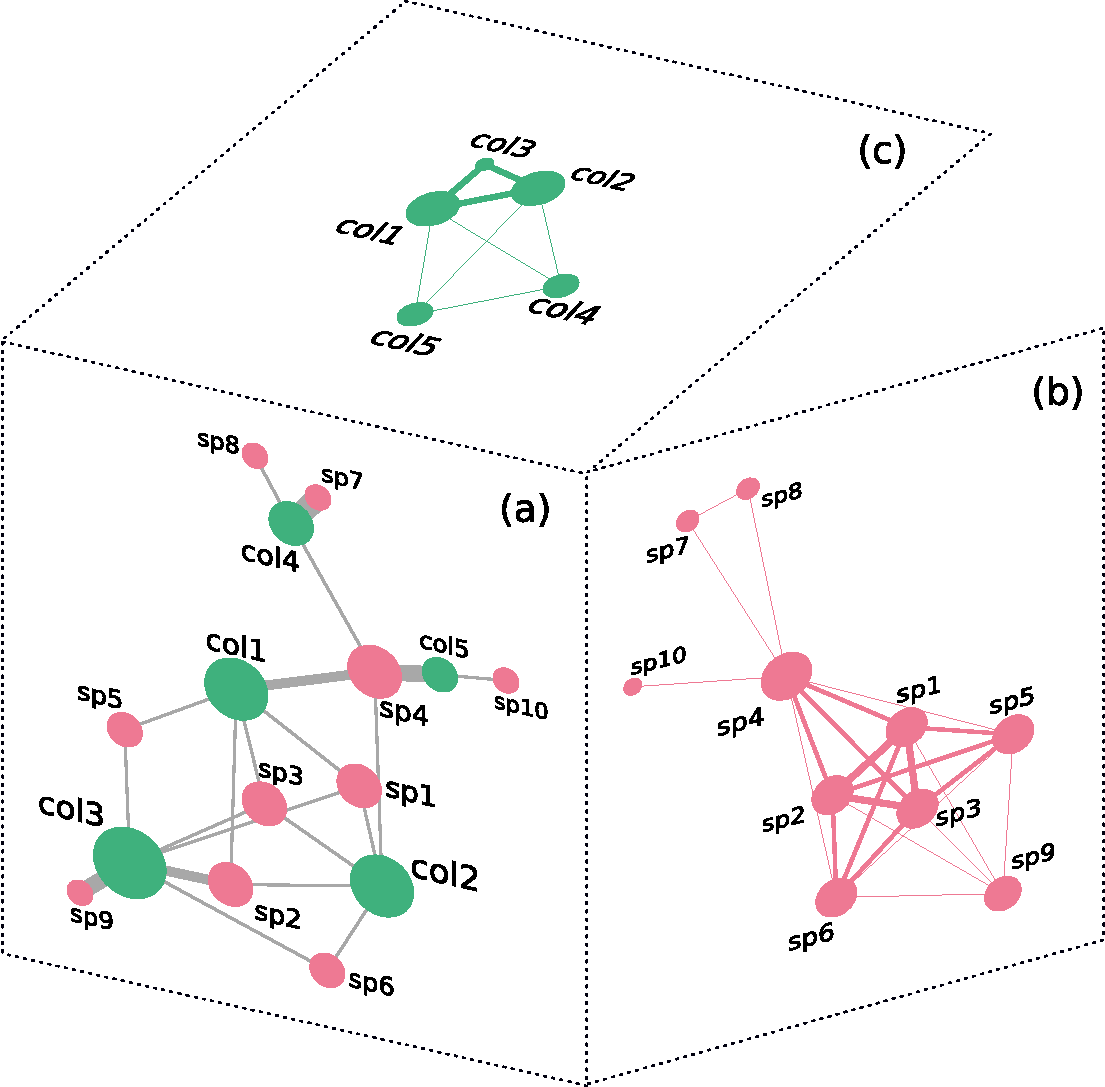
\includegraphics[width=.7\linewidth]{figures/network_models/scn_generalaspect.pdf}
    \caption{Multiple perspectives of a Species-collectors Network model (SCN).
    (a) Unprojected network, where collectors (green nodes) are linked to the species (red nodes) they've recorded. The total number of records of a given species by some collector is reflected in the strength of their link. (b) SCN projection onto the species set. Species are linked together if they've been collected by common collectors. Link strength is proportional to the number of collectors two species share. (c) SCN projection onto the collectors set. Collectors are linked together if they've recorded species in common. Link strength is proportional to the number of species two collectors share. 
    Link strength for both projections were obtained using the \textit{simple weighting} rule (eq. \ref{eq:simple_weighting}), and are graphically displayed as edges thickness. Nodes sizes reflect collectors' and species' degrees in each perspective.}
    \label{fig:scn_general}
  \end{figure}
  
%% Model specification
As collectors and species refer to distinct entities in our system, we represent them in our network as two disjoint nodes sets.
Moreover, as interest relationships here modeled can only possibly exist between collectors and species we impose an additional constraint that all edges in the network must necessarily connect nodes from distinct sets.
This best matches the description of a bipartite network
$$ SCN = (S_{col},S_{sp},E) \mbox{ ,}$$
where $S_{col} = \{u_1, u_2, ..., u_n \}$ is the nodes set representing the collectors group; $S_{sp}=\{v_1,v_2, ..., v_m\}$ is the nodes set representing the species group; and $E$ is the set of undirected edges between members of $S_{col}$ and $S_{sp}$.
The bipartite graph can also be represented as a rectangular biadjacency matrix $A^{n\times m}$ for which $a_{ij}\neq 0$ \textit{iff} $(u_i,v_j) \in E$. Values of non-zero $a_{ij}$ elements are set to the number of times edges $(u_i,v_j)$ occur in the network, as described below. 
For a general overview of bipartite graphs the reader should refer to section \ref{section:graphtheory}.

  
%% Network construction
\subsection{Model construction from data}
A SCN model is built from a species occurrence dataset by using basically two fields.
The first is the collectors field, containing the names of all collectors that were responsible for the record; and the second is the species field, storing the species identity assigned to the specimen in the record.
Following Darwin Core terms standard\footnote{\url{http://rs.tdwg.org/dwc/terms/}}, we should expect to find collectors names in the \textit{recordedBy} field; and the species name in a field named \textit{species}. As not every biological collection dataset uses Darwin Core standards though, these fields might be occasionally found under different names.

The network is built up from the dataset in an iterative process, in which weighted edges linking collectors to species are structured from rows in the dataset.
For each new record containing $n$ collectors, $n$ links connecting each individual collector to the recorded species are created (or strengthened, in case they already existed).
In the end of the process, the strength of each link is equivalent to the number of times each association appears in the original dataset.
The more often a particular collector records a particular species, the stronger gets the link between them.
Moreover, as at least one additional link is necessarily either created or reinforced for each new row, the construction process guarantees that no disconnected species or collector nodes can possibly exist in a species-collectors network.
For a concrete example, the dataset used for creating Figure \ref{fig:scn_general} is given in Table \ref{table:scn_example_dataset}.

\begin{table}[!ht]
  \caption{Species occurrence dataset from which the SCN model in Figure \ref{fig:scn_general} was built.}
  \begin{center}
  \begin{tabular}{r l c}
      id & recordedBy & species \\
      \hline
      0 & col1; col2; col3 & sp1 \\
      1 & col1; col2; col3 & sp2 \\
      2 & col1; col2; col3 & sp3 \\
      3 & col1; col2 & sp4 \\
      4 & col1 & sp4 \\
      5 & col1; col3 & sp5 \\
      6 & col3; col2 & sp6 \\
      7 & col3 & sp2 \\
      8 & col4 & sp4 \\
      9 & col4 & sp7 \\
      10 & col4 & sp7 \\
      11 & col4 & sp7 \\
      12 & col4 & sp7 \\
      13 & col4 & sp8 \\
      14 & col3 & sp9 \\
      15 & col3 & sp9 \\
      16 & col3 & sp9 \\
      17 & col5 & sp4 \\
      18 & col5 & sp4 \\
      19 & col5 & sp4 \\
      20 & col5 & sp10 \\
       \hline
  \end{tabular}
  \end{center}
  \label{table:scn_example_dataset}
\end{table}

We keep the record of the number of times each link occurs in the network by assigning a \textit{count} attribute to them, which is initially set to $1$ and is increased by one every time a new occurrence of the link is observed. Link strength is proportional to this attribute, and is graphically represented by edges thickness, as it can be observed in Figure \ref{fig:scn_general}.
Edges' \textit{count} values are stored in the biadjacency matrix $A$, and thus the value of element $a_{ij}$ is the number of times the edge $(u_i, v_j)$ occurs. 
The adjacency matrix for the example SCN network in Figure \ref{fig:scn_general} is thus
$$
A =
\kbordermatrix{
& sp1 & sp2 & sp3 & sp4 & sp5 & sp6 & sp7 & sp8 & sp9 & sp10 \\
col1 & 1 & 1 & 1 & 2 & 1 & 0 & 0 & 0 & 0 & 0 \\
col2 & 1 & 1 & 1 & 1 & 0 & 1 & 0 & 0 & 0 & 0 \\
col3 & 1 & 2 & 1 & 0 & 1 & 1 & 0 & 0 & 3 & 0 \\
col4 & 0 & 0 & 0 & 1 & 0 & 0 & 4 & 1 & 0 & 0 \\
col5 & 0 & 0 & 0 & 3 & 0 & 0 & 0 & 0 & 0 & 1 \\
}.
$$
An homonymous attribute is also set to graph nodes, which is increased whenever a new link involving the node is either added or strengthened. As a result the node's \textit{count} attribute keeps a record of how many times a given species or collector occurs in the dataset.
The reader should note, however, that \textit{count} attributes for nodes and edges are conceptually distinct and are not to be confused.


% SCN Definitions

\subsection{Definitions}
Given an overall description on the structure and semantics of the SCN model, we now define a set of attributes and operations that provide higher-level abstractions for dealing with the system here modeled. By using such field-domain abstractions we potentialize the data exploration process, eventually making it more insightful for the analyst.
We introduce both the \textit{species bag} and the \textit{quorum vector} as specific attributes of collectors and species.
Moreover, we define the process of taxonomy aggregation as a model summarization routine for grouping together species nodes into higher-rank taxa.

\paragraph{Species bag.} 
The entire set and counts of species a collector has recorded in a dataset, which can be thought as a collector's species signature, composes his/her \textit{species bag}. This attribute is therefore exclusively derivable for collectors nodes.
As species bags are directly obtained as row-vectors of the graph's biadjacency matrix, they are a convenient structure for comparing collectors in terms of the composition of their records.
For that task a high variety of well-known distance algorithms for vectors in literature can be readily applied.
The species bag $\sigma$ for collector $u_i$ is defined as

$$
\sigma_{u_i} =  \begin{bmatrix}
a_{i 1}, a_{i 2}, ..., a_{i m}
\end{bmatrix}  \quad ,
$$
where $m$ is the length of the species set and each $a_{i j}$ is the total number of records of species $v_j$ by collector $u_i$. The sum of all elements in a collector's species bag, which is equivalent to the vector's \textit{l1 norm} $||\sigma_{u_i}||_1$, corresponds to the total number of records for that collector.

 
\paragraph{Quorum.} 
The entire set and counts of collectors who have recorded a particular species in a dataset comprise its \textit{quorum}, an exclusive attribute of species nodes. 
This concept can be thought as the inverse of a species bag, being the collectors signature of a species. 
The quorum vector $\iota$ of a species $v_j$ is directly obtained from the graph's biadjacency matrix as the $j^{th}$ column-vector 

$$
\iota_{v_j} = \begin{bmatrix}
a_{1 j}, a_{2 j}, ..., a_{n j}
\end{bmatrix} \quad ,
$$
where $n$ is the length of the collectors set and each $a_{i j}$ is the total number of times collector $u_i$ has recorded species $v_j$. 
The total number of occurrences of species $v_j$ in the entire dataset can be obtained as the sum of all elements in its quorum vector $ || \iota_{v_j} ||_1$.


\paragraph{Taxonomic aggregation and resolution.}\label{section:taxonomic_aggregation}
In some contexts it might be desired to simplify SCNs by grouping species nodes into higher taxonomic ranks (or levels), such as \textit{genus} or \textit{family}. This process is defined as \textit{taxonomic aggregation}, and is performed by 
($i$) obtaining a grouping of species using some taxonomic rank; 
($ii$) obtaining quorum vectors for each species; 
($iii$) summing up quorum vectors for all species in each group;
($iv$) building a new SCN model, aggregated on rank T. 
The SCN's \textit{taxonomic resolution} is the taxonomic rank at which species are aggregated in the model. For the sake of model interpretability, all nodes in $S_{sp}$ must necessarily be represented as taxons belonging to the same rank as the SCN's taxonomic resolution.

For a more formal description let $G_T = \{g_1,g_2,..., g_n\}$ denote a taxonomic grouping at rank $T$, containing a set of $n$ rank-$T$ taxa.  In addition, let each taxon $g_i \in G_T$ itself be a set of nodes $S_{sp}^{(i)} \subseteq S_{sp}$, with the conditions that there are no empty $S_{sp}^{(i)}$ and that every node $v \in S_{sp}$ is a member of exactly one set  from $ \{ S_{sp}^{(1)}, S_{sp}^{(2)}, ..., S_{sp}^{(n)} \}$.
Such a grouping rule makes $G_T$ a partition of $S_{sp}$, and thus the entire set $S_{sp}$ can be recreated by simply computing the union of elements in $G_T$. This guarantees that no entities are duplicated or eliminated on aggregations using it.

We then use grouping $G_T$ for obtaining quorum vectors for each of its taxa $g_i \in G_T$, which will be represented as nodes in the new aggregated graph. Quorum vectors are computed as $ \iota_{g_i} := \sum_j \iota_{v_j}  $ for $v_j \in S_{sp}^{(i)}$. Finally, the rank-$T$ aggregated  graph $SCN_T=(G_T,S_{col},E)$ is created from a biadjacency matrix, which is constructed by stacking quorum vectors for each taxon $g_i$ as row-vectors. The set of collectors nodes remain the same in the aggregated graph.

% The PICI model (Lambiotte2005)
%% Collective effects acting on individuals with similar interests
%% Individual mechanisms, pushing collectors towards their particular interests, establishing their collecting niche

% Temporal edges


% SCN projections
\subsection{Projections} \label{section:scn_projection}

Bipartite projections on each one of the SCN's nodes sets allows one to investigate indirect associations two entities from the same class might have with each another, as intermediated by a third entity from the opposite class. 
Figure \ref{fig:scn_general} illustrates projections of a SCN onto the species set (b) and the collectors set (c).
In overall, each projection gives us complementary perspectives of transitive relationships in the SCN, either from the collectors or species point of view.

From a \textit{species-centric perspective} (Figure \ref{fig:scn_general}b), connections are formed between species having been recorded by at least one collector in common, with link strength proportional to the number of different collectors they share. 
Although collectors are used during projection for determining the existence of links between species they are not represented as nodes in this projection.
In general strongly connected species can be interpreted as being both included in the species bags of many collectors, whereas weakly connected or isolated species are seldom or never recorded by the same collectors.
% Modules in species projections reveal species that are more intensely associated with each other than with others from outside the module
The second perspective (Figure \ref{fig:scn_general}c) is \textit{collectors-centric}, in that only collectors are represented as nodes whilst species are omitted. 
Analogously to the species-centric perspective, here collectors are linked together if they have recorded at least on species in common, with link strength depending on the number of shared species between them. 
From this perspective we could identify collectors having similar recording profiles.

As previously discussed in this text, projections are a mechanism for summarizing bipartite into more convenient one-mode graphs, where only one class of entity is represented. 
Projections, however, come with the cost of information loss, as any relationships or attributes of nodes from the omitted set are not represented in the projection \cite{Borgatti1997}. 
Moreover, relevant associations between entities eventually become obfuscated by others of lower relevance, as projections tend to generate graphs that are much denser than the original bipartite model \cite{Lambiotte2005}.
Choosing an appropriate weighting rule for the aspects one wants to investigate is thus crucial for separating relevant from less-relevant associations, so that the latter ones can be subsequently removed by applying weighting filters.
Below I first describe the simplest weighting rule with its limitations and, in sequence, some alternatives rules for overcoming them.
% https://doi.org/10.1016/j.physa.2006.12.021 <- The effect of weight on community structure of networks

\paragraph*{Simple weighting.}
This rule assigns weights to links between pairs of collectors ($u_s$ and $u_t$) or species ($v_s$ and $v_t$) by simply counting the total number of species collectors share on their species bags or the total number of collectors species share in their quorum vector. The rule is mathematically expressed as:
\begin{equation} \label{eq:simple_weighting}
\begin{split}
w_{(u_s, u_t)} &= \sum_{j=1}^{m} \delta(\sigma^{(j)}_{u_s}, \sigma^{(j)}_{u_t})\mbox{ , for the projection onto }S_{col}\mbox{ ;}\\
w_{(v_s, v_t)} &= \sum_{i=1}^{n} \delta(\iota^{(i)}_{v_s}, \iota^{(i)}_{v_t})
\mbox{ , for the projection onto }S_{sp}\mbox{, where}
\end{split}
\end{equation}
$n = |S_{col}|$, $m = |S_{sp}|$, $\sigma^{(i)}$ and $\iota^{(i)}$ are the $i^{th}$ element of a species bag and a quorum vector, respectively; and $\delta(u,v)=1$ if both $u$ and $v$ are non-zero and $0$ otherwise.

In order to obtain the weights for every pairs of projected nodes more efficiently we can use a vectorized implementation of this rule. First we derive a $n\times m$ logic matrix $A_{bool}$ from the SCN biadjacency matrix $A$ by simply replacing its non-zero elements by ones. 
Then a $n \times n$ adjacency matrix with edges weights for the $S_{col}$ projection is obtained by calculating the dot product $A_{bool} A_{bool}^T$.
Conversely, for the $S_{sp}$ projection, the $m \times m$ weights matrix is obtained by calculating $A_{bool}^T A_{bool}$.

The simple weighting rule has an important limitation when applied to SCNs.
It arises from the fact that the weight assigned to edges linking pairs of nodes in the projection only reflects the number of distinct intermediate neighbors from the complementary set they shared in the non-projected graph. The number of times each species is recorded by each collector is therefore ignored while computing the strength of links in the projections, underestimating the importance of recurrent relationships.
Consequently this weighting rule tends to make very prolific and generalist collectors or very attractive species strongly connected to many others in a disproportional way, as an effect of their high degrees in the non-projected model. The opposite happens in the case of specialized nodes, which typically hold fewer --- although recurrent --- distinct links to their neighbors. 
In order to reduce these effects two alternative rules are proposed below.

\paragraph*{Additive weighting.}
This rule is a slight modification of the simple weighting rule, in that it also considers the total number of times entities interact through each neighbor-intermediated path in the non-projected network. The rule is expressed using the same equations from (\ref{eq:simple_weighting}), but changing the $\delta$ function to
 
$$\delta(u,v) = 
\begin{cases}
\frac{u+v}{2} &  \mbox{if both } u \mbox{ and } v \mbox{ are non-zero ,}\\
0 & \mbox{otherwise}
\end{cases}
$$
In case every distinct path in the non-projected SCN only occur once then both simple and additive weighting rules lead to the same result. % TODO: Test this assumption 
This modified rule potentializes the effect of recurring edges from the non-projected graph on computing edges weights in the projection, thus reducing weighting asymetries from generalist and specialized nodes.

However, this approach still has a drawback in that nodes which have high degrees in the non-projected graph tend to become much more strongly connected with themselves in the projection than average-degree ones, simply by the fact that they have many more connections than average.
Additionally, without a superior limit for the $\delta$ function it turns out to be hard to determine a proper threshold when filtering relevant from non-relevant edges. The next weighting rule is designed to reduce the effects of nodes degrees on their edges' weights, outputting values which are bounded to the $[0,1]$ interval.

\paragraph*{Species bag / Quorum similarity.}
% This is called "Structural Equivalence": Nodes have ties to common third-parties {Borgatti2015}
% One characteristic is that in practice collectors holding similarity values very close to one tend to be those with very few records in the dataset. More experienced collectors can have higher similarities with some collectors, but it is usually not very high.
This weighting rule uses a similarity (or correlation) matrix that is computed for each projection of the SCN. Edges' weights are given by the similarity between their nodes. The similarity matrix for the collectors and species projections are constructed by computing the  \textit{cosine similarity} of species bags and quorum vectors  for each pair of nodes in the respective projection. 
The \textit{species bag similarity} for collectors $u_s$ and $u_t$; and the \textit{quorum vector similarity} for species $v_s$ and $v_t$ are defined as

\begin{equation}
\label{equation:cosine_similarity}
\begin{split}
sim(\sigma_{u_s},\sigma_{u_t}) &\equiv
\cos \theta_{u_s,u_t} =
\frac{  \sigma_{u_s} \cdot \sigma_{u_t}  }{  ||\sigma_{u_s}||_2  ||\sigma_{u_t}||_2  } \\
sim(\iota_{v_s},\iota_{v_t}) &\equiv
\cos \theta_{v_s,v_t} =
\frac{  \iota_{v_s} \cdot \iota_{v_t}  }{  ||\iota_{v_s}||_2  ||\iota_{v_t}||_2  } 
\end{split}
\end{equation}

Therefore each element in the similarity matrix holds the edge weight for a pair of nodes, with a value ranging within the interval $[0,1]$. Edges weights are zero-valued if no direct link exist between two nodes,  whilst nodes linked by edges with a weight of $1$ have identical species bags or quorum vectors. Intermediate values reflect the correlation measure obtained for node pairs.
As this rule outputs weight values that are bound to a known interval, filtering less relevant links becomes much more straightforward. Depending on the aspects regarding the species-collectors system an investigator might be interested in, a filtering threshold $\phi$ can be set based on the minimum correlation value she considers acceptable, such that only the most relevant relationships for that particular analysis are kept.
%%% check neighborhood similarity functions in literature
%% Edges pruning












% =============================
% =============================
% Collectors Coworking Networks
% -----------------------------
%
% As in this model it is possible for even for collaborative collectors to record some records alone, the weighted degree is not necessarily equivalent to his/her total number of records. Instead, it is equivalent to his/her total number of collaborative records.

\section{Collectors Coworking Networks}
In this section we describe collector coworking networks (CWNs) as modeling collaborative associations between collectors.
We first define CWNs using graph theory and then we describe how such models can be structured from species occurrence datasets.

\subsection{General Description}
\textbf{Collector Coworking Networks} are a particular instance of \textit{collaboration networks} describing coauthoring relationships between collectors from species occurrence records (Figure \ref{fig:cwn_general}).
We consider two collectors to be coauthors in a given record if they are both included in the collectors field for that record. The collectors field holds a list collectors names who have authored each record in the dataset, and is equivalent to the \textit{recordedBy} field in a dataset following \textit{Darwin Core} terms standards (check an example in Table \ref{table:cwn_example_dataset}). We refer to each distinct list of collectors in this context as a \textbf{team}.

As opposed to SCNs, which describe collectors interests towards species, relationships in CWNs are directly formed between collectors who have effectively worked collaboratively in field, and are semantically described as ``\textbf{collector} records specimen with \textbf{collector}''.
Each individual species occurrence record with at least two collectors (team size greater than $1$) is thus considered a distinct collaboration act, originating new pairwise connections between all collectors involved.
For records with team size equal to $1$, which we refer to as non-collaborative records, no connections are created.

  \begin{figure}[h!]
  	\centering
    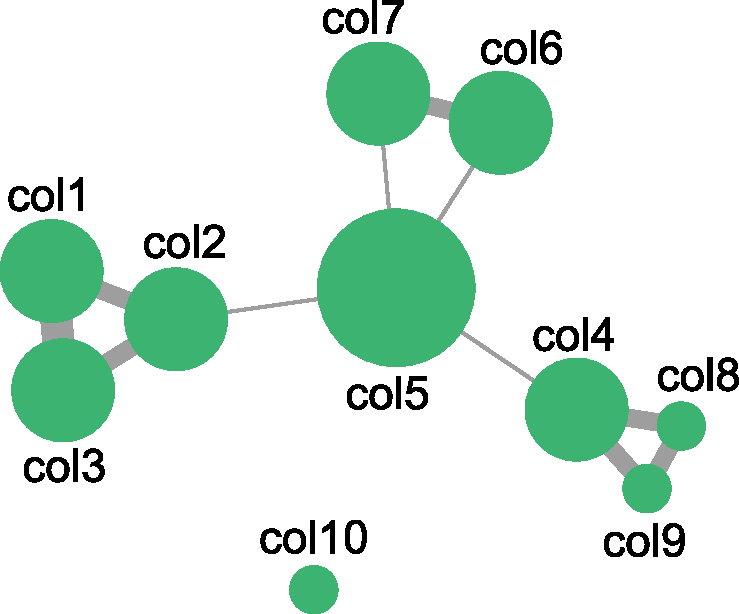
\includegraphics[width=.4\linewidth]{figures/network_models/cwn_generalaspect.pdf}
    \caption{General aspect of a Collectors Coworking Network (CWN). Coauthoring relationships between collectors (green nodes) are structured as edges in the graph, and are graphically represented as gray links.
    Here collectors nodes are sized according to the total number of records they've authored; and edges are weighted according to the number of collaborative records coauthored by both nodes.}
    \label{fig:cwn_general}
  \end{figure}

Differently from SCNs, where two entities classes are represented in the graph as disjoint nodes sets with the bipartite constraint, CWNs exclusively model direct relationships between entities from a single class (collectors), with the only connectivity restriction that a collector should not hold collaborative ties to itself.
The model is thus formally described as an unipartite (or one-mode) undirected graph
$$CWN = (S,E) \mbox{ ,}$$
where $S=\{u_1,u_2,...u_n\}$ is the graph's nodes set and $E$ is the set of undirected edges linking members of $S$.

Analogously to SCNs, both nodes and edges hold homonymous but conceptually distinct \textit{count} attributes.
Nodes count attribute stores the total number of records --- including non-collaborative ones --- a collector has authored, whereas
edges count attribute stores the total number of times an association between two collectors was observed in the dataset. Thus, although each node and edge respectively are uniquely included in $S$ and $E$, their recurrence patterns are registered in the model as attributes.
Another important edge attribute is the \textit{species list}. Although species associated to each occurrence record are not represented as entities in this model, edges can optionally keep a list of species that are shared by two collectors through that link, which is stored in this attribute.

Weights are assigned to edges in the CWN as a measure of their overall relevance in the network structure. Edges with higher weight values represent stronger collaborative ties between collectors, pointing out the main groups of collectors who are most willing to collaborate. 
The simplest rule is to set the edge weight as the total total number of occurrences of the tie it represents in the dataset. However, as pointed out by other authors studying social networks \cite{Newman2001a}, in reality not all collaboration acts should contribute the same way for a collector's network. 
Collectors tend to hold weaker collaborative ties with each other when they collaborate in larger teams than when they collaborate in smaller ones. 

The \textbf{hyperbolic weighting} rule accounts for this fact, while also considering the total number of collaborations between two collectors as a factor contributing the strength of their link.
According to this rule, not every new occurrence of the link increases the edge weight equally. 
The contribution of each new link depends on the number of the collectors $n^{(k)}$ included in record $k$ or, in other words, the team size. 
This rule follows a hyperbolic growth function 
\begin{equation}
w_{(i,j)} = \sum\limits_k \frac{\delta_i^{(k)} \delta_j^{(k)}}{(n^{(k)}-1)} \mbox{ , }
\end{equation}
where $\delta^{(k)}_u = 1$ if collector $u$ is in record $k$ and $0$ otherwise.
As the hyperbolic function above has singularity at $1$, it gets ill-defined for records with only one collector. 
Therefore only records with two or more collectors are used to compute edges weights. 
The maximum weight contribution of 1 is assigned to records with two collectors, whilst records with larger cliques yield smaller contributions.\\

Relationships in the CWN graph can be represented in a symmetric adjacency matrix $A^{n\times n}$ for which $a_{ij} \neq 0 \textit{ iff } (u_i,u_j) \in E$. 
Values of non-zero elements depend on the weighting method adopted for representing links strength, being the absolute counts of edges' recurrence (edges' \textit{count} attribute) the simplest one.
Additionally, the model's connectivity constraint states that all diagonal elements in $A$ are necessarily equal to $0$, thus ensuring that no self loops are formed.
To give a concrete example, the adjacency matrix for the graph in Figure \ref{fig:cwn_general} is 
$$
A =
\kbordermatrix{
& col1 & col2 & col3 & col4 & col5 & col6 & col7 & col8 & col9 & col10 \\
col1 & 0 & 2 & 2 & 0 & 1 & 0 & 0 & 0 & 0 & 0\\
col2 & 2 & 0 & 3 & 0 & 0 & 0 & 0 & 0 & 0 & 0\\
col3 & 2 & 3 & 0 & 0 & 0 & 0 & 0 & 0 & 0 & 0\\
col4 & 0 & 0 & 0 & 0 & 1 & 0 & 0 & 2 & 2 & 0\\
col5 & 1 & 0 & 0 & 1 & 0 & 1 & 1 & 0 & 0 & 0\\
col6 & 0 & 0 & 0 & 0 & 1 & 0 & 2 & 0 & 0 & 0\\
col7 & 0 & 0 & 0 & 0 & 1 & 2 & 0 & 0 & 0 & 0\\
col8 & 0 & 0 & 0 & 2 & 0 & 0 & 0 & 0 & 2 & 0\\
col9 & 0 & 0 & 0 & 2 & 0 & 0 & 0 & 2 & 0 & 0\\
col10 & 0 & 0 & 0 & 0 & 0 & 0 & 0 & 0 & 0 & 0
},
$$
where each element is the count of the total number of recurrences of collectors associations, represented in the graph as edges weights.




% Network construction
%% Singleton collectors are those holding no collaborative recording with any other collector in the dataset ($k=0$), and are also included in the model as isolated nodes.
\subsection{Model construction from data} \label{section:cwn_construction_fromdata}

We build CWNs from species occurrence data in an iterative process that is similar to the one described for SCNs.
In this case, however, the only field that is strictly required for structuring relationships is the one containing collectors names, which in a database following \textit{Darwin core} terms standards should be named ``\textit{recordedBy}''.
The field containing species identities, although not required, can be optionally used during model construction in case the user decides to set the edges' \textit{species list} attribute.
Table \ref{table:cwn_example_dataset} shows the species occurrence dataset which was used to build the graph in Figure \ref{fig:cwn_general}.

\begin{table}[!ht]
  \caption{Species occurrence dataset from which the CWN model in Figure \ref{fig:cwn_general} was built. The \textit{species} field is not strictly required for building CWN models.}
  \begin{center}
  \begin{tabular}{r l c}
      id & recordedBy & species \\
      \hline
        0 & col1; col2; col3 & sp1\\ 
        1 & col3; col1; col2 & sp2\\ 
        2 & col1; col3 & sp3\\ 
        3 & col5; col4 & sp3\\ 
        4 & col5; col2 & sp3\\ 
        5 & col5; col6 & sp5\\ 
        6 & col5; col7 & sp4\\ 
        7 & col6; col7 & sp6\\ 
        8 & col6; col7 & sp7\\ 
        9 & col4; col8; col9 & sp4\\ 
        10 & col4; col9; col8 & sp5\\ 
        11 & col10 & sp6\\ 
        12 & col10 & sp6\\
       \hline
  \end{tabular}
  \end{center}
  \label{table:cwn_example_dataset}
\end{table}

For each row in the dataset, a \textit{clique} structure is formed by creating edges between all collectors included in the record's team, in a pairwise fashion. 
Each clique thus represents one collaborative act, where every collector gets and additional collaborative tie with every other collector included in that collaborative record. 
The clique size, which is the number of nodes included in the clique structure, is equivalent to the team size. For non-collaborative records the clique is composed by the collector node itself, and therefore no edges are formed.
As the user might want to distinguish the relevance of links originated from distinct team sizes, the hyperbolic weighting rule described in the previous section can be used for weighting links in each clique. 
In case the species field is included in the building routine, each clique also gets associated to the name of the species to which the recorded specimen belongs to.

The CWN model is finally composed by combining all cliques together into a single undirected graph. In this process edges that occur in multiple cliques have their weights summed. In case the species list attribute is set, combining edges also merges their respective species lists.




% Are unconnected collector represented in the model?
%% Average number of collaborators?


%% Weighting
%%% Check the weighting rule from Newman2001a -> Hyperbolic weighting
